\begin{frame} [fragile]
	\frametitle{TOF-wall detector}
	\begin{columns}
  		\begin{column}{0.50\textwidth}
            \begin{itemize}
                \item TW used to \textcolor{blue}{measure the energy loss} $\Delta$E of the passing particles and to provide their arrival time.
                \item Made of \textcolor{blue}{40 bars} of EJ-200 plastic scintillator arranged in two orthogonal layers of 20 each.
                \item At each end of each bar, the two series of two \textcolor{blue}{SiPMs} were connected in parallel.
            \end{itemize}
		\end{column}
    \begin{column}{0.50\textwidth}
 		\newline
			\begin{figure}
	  		    \centering
				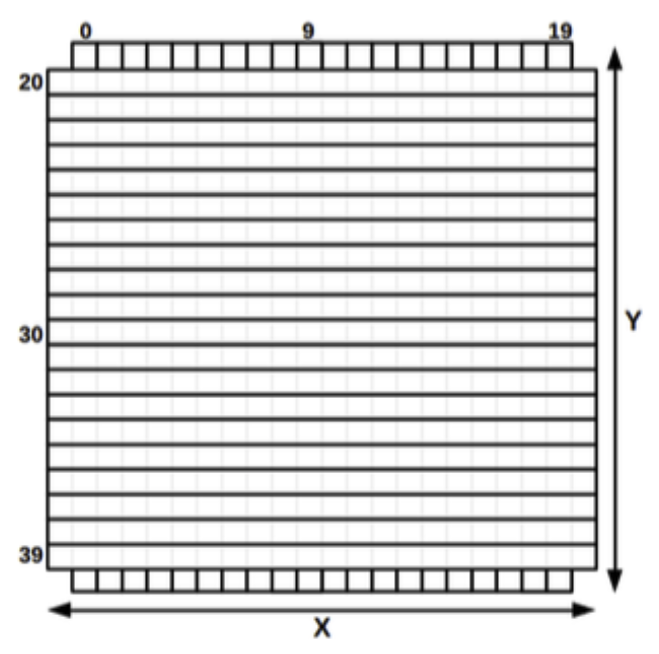
\includegraphics[scale=0.15]{figures/tof_wall_scheme.png}
				%\caption{Spettri energetici di diversi ioni nei GCR \cite{saggiatore}}
                \caption{Scheme of TOF-Wall bar numbering}
			\end{figure}
    \end{column}
\end{columns}
\end{frame}